%-required
\documentclass[UTF8,no-math]{ctexart}
\AtBeginDocument{\usepackage[l2tabu, orthodox]{nag}} %correct package use
\usepackage{geometry} %Use \geometry to modify the page size
%\usepackage{ctex} %disable if write in English
\usepackage{amsmath}
\usepackage{xfrac} %\sfrac
\usepackage[table]{xcolor}%colored text or box, or even table (\cellcolor)
\usepackage[normalem]{ulem} % \sout{1234} to generate delete lines, and \uline for continous underlines.
\usepackage{bm} %use \bm to create bold math style.
\usepackage{upgreek} %\use \uppi to get const pi.
\usepackage{mathtools}%dcases, \overbracket, \prescript, \shortintertext
\usepackage{graphicx} %To use \includegraphics
\usepackage{booktabs}%use \toprule \midrule \bottomrule
\usepackage{siunitx} %use \SI to display units.
\usepackage{enumerate} %use \begin{enumerate} and \item
\usepackage{enumitem} %detailed adjustments for enumerate
\usepackage{caption}%detailed adjustments to captions
\usepackage{subcaption}%use subtable or subfigure environment
\usepackage{float}%use \begin{table}[H] to get non-float boxes
\usepackage{bdm2}

%-optional
\usepackage[lf,minionint,mathtabular]{MinionPro}%Lining Number and favorite Minion Pro!
\usepackage{fontspec}
\setmainfont{Minion Pro}

\usepackage{pgfplots}%to draw!!!
%\usepgfplotslibrary{polar}%to use \begin{polaraxis}!!
\usepackage[all,pdf]{xy}
\usepackage[inline]{asymptote}
\usepackage{esvect}%use \vv to produce a right arrow above.
\usepackage{multirow}%use \multirow{n}{*}{sth} to combine n cells in a single col
\usepackage{makecell}% to use '\\' in table cells.
%to combine n cells in a single row of a table, use \multicolumn{c}{n}{sth}
\usepackage{diagbox}
\usepackage{pdfpages}%use \includepdf[pages={1}]{*.pdf} to insert pdf
%\usepackage{pdflscape} %use landscape environment with pdflatex
%\usepackage{ragged2e} % RaggedLeft, justify
\usepackage{framed}
\usepackage[version=4]{mhchem} %use \ce to produce chemical equations
\usepackage{lipsum}%use \lipsum[num] to create random text
%\usepackage{framed} %framed environment can create boxes

\usepackage{multicol}%use \begin{multicols}{n} to divide the page
%\usepackage{cases}%use \numcases to build multiline equations with labels
\usepackage{galois}%use \comp to g·y
\usepackage{extarrows}%use \xlongequal
\usepackage{mathrsfs}%use \mathscr{E} to get the symbol of electromotive force 'E'
\usepackage{fontawesome} % frontend engineers have cried!
\usepackage{listings}%\begin{lstlistings}[language=C] coding...syntax \end{lstlistings} 
\usepackage{hyperref} % \href{URL}{text} and \url{URL}
\usepackage{nameref} % \nameref{label} to get ref name
\usepackage{lastpage} %\pageref{LastPage} to get page number of the last page
%\usepackage{breqn} %dmath envirn can split quations autoly, with bug
%\usepackage{syntonly}\syntaxonly % check syntax without building

%-XUANology
\usepackage{microtype}


%-if references are required, enable these two lines and edit ref.bib. cite with \cite{}
%\usepackage[backend=biber,sorting=,style=,]{biblatex}
%\addbibresource{ref.bib}


%-package config
\usepgfplotslibrary{external} % Automatic externalization. -shell-escape should be added to compiling command.
\tikzexternalize

\pgfplotsset{compat=1.16}
\sisetup{range-phrase=-,%
    group-digits=false,%
    list-pair-separator={, },%
    list-final-separator={, },%
    binary-units=true,% like \mebi or \gibi
}
\captionsetup{labelsep=quad,
    font+={small},
    labelfont+={bf},
    margin=4em,
    figurename=图,
    tablename=表,
}
\renewcommand{\figureautorefname}{图}
\renewcommand{\tableautorefname}{表}
%\geometry{a4paper, top=2.54cm, right=3.18cm, bottom=2.54cm, left=3.18cm} %enable if want a page identical to Microsoft Word A4
\mhchemoptions{layout=stacked}%eable if use mhchem
%\newfontfamily\consolas{Consolas}%新的等宽字体族
\setlength{\columnseprule}{.4pt}
\lstset{%enable if use listings
	numbers=left, 
	numberstyle= \footnotesize, 
    basicstyle=\ttfamily, 
	keywordstyle= \bfseries,
	commentstyle= \itshape\color{red!50!green!50!blue!50}, 
    stringstyle=\sffamily\bfseries\color{blue},
	frame=shadowbox, % 阴影效果
	rulesepcolor= \color{ red!20!green!20!blue!20},
	breaklines,%自动换行
    escapechar=',%设置抑音符为转义字符. 但我不晓得它为什么不起作用.
	columns=flexible,
}
\newtheorem{theorem}{定理}
\newtheorem{inference}{推论}[theorem]
\newcommand{\D}{\displaystyle}
\newcommand{\T}{\textstyle}

% length adjustments
\setlength{\lineskiplimit}{2.625bp}
\setlength{\lineskip}{2.625bp} % provent a text line with high contents like \dfrac reach too close to adjacence.

% macro definations
\makeatletter
\newcommand{\hl}[1]{\colorbox{yellow}{#1}} %需要更好的实现
\makeatother

%document-use package and settings
\usepackage{metalogo}
\numberwithin{enumi}{section}
\setlist[enumerate,1]{label=\textbf{\theenumi}}
\pagestyle{headings}

%-prebody

\hypersetup{
    pdftitle={bdm 与 LaTeX 使用范例},
    pdfauthor={me@beardic.cn},
    pdfcreator={XeLaTeX+xeCJK+TikZ+XYpic+Asymptote},
    pdflang={Chinese},
}

\title{bdm 与 \LaTeX{} 使用范例\footnote{参考文献: 刘海洋. \emph{\LaTeX 入门}[M]. 第 1 版. 北京:电子工业出版社, 2013-6.}\\—— \LaTeXe{} 无极限}
\author{Dict Xiong\thanks{共同第一菜鸡.}\\清华大学 \and Bear Dic\footnotemark[2] \\华清大学}
\date{\today}

%-body
\begin{document}
    \maketitle
    \begin{abstract}
        这是一段摘要示例. 就我个人来说, 摘要对我的意义, 不能不说非常重大. 生活中, 若摘要出现了, 我们就不得不考虑它出现了的事实. 一般来讲, 我们都必须务必慎重的考虑考虑. 池田大作说过一句富有哲理的话, 不要回避苦恼和困难, 挺起身来向它挑战, 进而克服它.
    \end{abstract}
    \tableofcontents\newpage
    \setcounter{section}{-1}
    \section{编译环境}
    这篇文章由 Windows 10 平台上的 \TeX Live 2019 发行版中的 \XeLaTeX 编译完成. 文章使用了外部引入的宏包 \texttt{MinionPro} (\url{https://www.ctan.org/pkg/minionpro}) 和 Minion Pro 字体族文件, 以及自定义宏包 \texttt{bdm2}. 编译时, 加入了参数 \verb|-shell-escape|.
    
    \section{基础文本}\label{sec:1st}
    这是一段平凡文本. 了解清楚正文到底是一种怎么样的存在, 是解决一切问题的关键. 现在, 解决正文的问题, 是非常非常重要的. 所以, 这种事实对本人来说意义重大, 相信对这个世界也是有一定意义的.  
    
    对我个人而言, 正文不仅仅是一个重大的事件, 还可能会改变我的人生. 我们一般认为, 抓住了问题的关键, 其他一切则会迎刃而解. 现在, 解决正文的问题, 是非常非常重要的. 
    \begin{bdquote}[indent]
        这是一段引用示例. 如果指定可选参数为 \texttt{indent}, 那么将会首行缩进, 否则不缩进. 
        
        引用因何而发生? 在这种困难的抉择下, 本人思来想去, 寝食难安. 问题的关键究竟为何? 引用, 发生了会如何, 不发生又会如何. 既然如何, 引用, 发生了会如何, 不发生又会如何. 了解清楚引用到底是一种怎么样的存在, 是解决一切问题的关键. 
        
        Lorem ipsum dolor sit amet, consectetur adipiscing elit. Aenean faucibus eros sed mi volutpat feugiat. Donec tincidunt, mauris id convallis mattis, neque massa dignissim tortor, sit amet tempus enim erat sed tortor.
    \end{bdquote}
    \begin{enumerate}
        \item 关于文档类的选择, 刘海洋认为: (\url{https://www.zhihu.com/question/58656895})
        \begin{bdquote}[indent]
        全中文的文档,尽量用 \texttt{ctex} 文档类。也就是 \texttt{ctexart}、\texttt{ctexrep}、\texttt{ctexbook}、\texttt{ctexbeamer} 这些。(如 \verb|\documentclass{ctexart}|)
        
        比较少见的情形下,你需要在某个原本不支持中文的文档类中写全中文的文档,此时用 \texttt{ctex} 包(\verb|\usepackage{ctex}|)。实际的例子,如用 \texttt{moderncv} 写简历。
        
        英文文档中的几段中文,建议用 \verb|scheme=plain| 选项调用 \texttt{ctex} 包,即\\ \verb|\usepackage[scheme=plain]{ctex}|。
        
        英文文档中的几个汉字(比如人名),建议把汉字做成图片,插图,这样不需要限定编译方式。如果允许用 \XeTeX 或 \LuaTeX,也可以直接切成汉字字体写中文,不加中文相关宏包。    
        \end{bdquote}
        \item 一个短横线 \texttt{-} 用于连字符, 两个短横线 \texttt{--} 表示数字范围, 三个短横线 \texttt{---} 表示破折号.
        \item 引号的使用. \par \emph{``\,`压缩' 这个词已经不仅仅限于它原本的意思了.'' 他说.}
        \item 西文省略号: 在句中时前后应有空格, 在句尾应当使用四个点. \par \emph{She $\ldots$ she got it. I've no idea\ldots. }
        \item 以字母命名的宏, 后面的空格会被忽略, 有些时候应避免.\par \emph{\LaTeX{} makes perfect. {\LaTeX} makes perfect. \sout{\LaTeX makes perfect.}}
        \item 西文句末后间距会比单词间距要大, 而 \LaTeX{} 判断的条件是句点前的字母是否为大写. 这个判断不一定正确, 因此要手动调整. \par \emph{Tinker et al.\ made the double play. World war II\@. Yes it is.} --- Correct. \par \emph{Tinker et al. made the double play. World war II. Yes it is.} --- Wrong.\par \uline{\fangsong 注}: 测试中, 中文行文使用英文句点, pdf\LaTeX 误判为句中, \XeLaTeX 则能正确判断句末. \textcolor{gray}{\sout{\faExclamationTriangle 这个问题的影响恐怕有点大.}} 我已经解决了. 从此告别 pdf\LaTeX. 
        \item 因此此处加一条. \XeLaTeX 会自动控制中英文间的间距. 如果要去掉空格, 可以用盒子. \par \emph{\mbox{矩形}a和矩形b是一样的.}\par 此外, 还可以用 \texttt{\textbackslash CJKsetecglue\{\}} 来修改中英文间字符 (默认是空格).\par \emph{\CJKsetecglue{-} 矩形a 和矩形b是一样的.}
        \item 断词. 默认情况下, \LaTeX\ 自动断词功能已经足够, 但是一些特殊单词可能无法正确处理. 在单词中使用 \verb|\-| 可以手动指定可能的断点, 还可以在导言区全局地设定断点列表, 如\par
        \verb|\hyphenation{man-u-script com-pu-ter}|
        \item 段落对齐方式. 默认为两端对齐, 另有左对齐 \verb|\raggedright|\footnote{这在窄英文段落中特别有用.}, 右对齐 \verb|\raggedleft|, 居中 \verb|\centering|. 对应环境 \verb|flushleft|, \verb|flushright|, \verb|center|. \par 
        使用非两端对齐的段落不会断词. 使用 \texttt{ragged2e} 宏包, 使用 \verb|\RaggedRight|, \verb|\RaggedLeft|, \verb|Centering| 以及 \verb|FlushLeft|, \verb|FlushRight|, \verb|Center| 环境可以保留断词, 更为合理. 其还提供了 \verb|\justifying| 和 \verb|justify| 环境, 可以还原两端对齐. 
        \item 字体族:\enspace{\ttfamily \textbackslash rmfamily, \textbackslash sffamily, \textbackslash ttfamily}\\
        字体系列:\enspace{\ttfamily \textbackslash mdseries, \textbackslash bfseries}\\
        字体形状:\enspace{\ttfamily \textbackslash upshape, \textbackslash itshape, \textbackslash slshape, \textbackslash scshape}
        \item \texttt{ulem} 宏包提供的一些功能.\par  
        {\itshape \uline{underline} \uuline{double underline} \uwave{wave underline} \sout{delete line} \xout{remove lines} \dashuline{dashed underline} \dotuline{dot underline}}
        \item 水平间距的一些例子. \par
        {\ttfamily \textbackslash hspace\{2em plus 1em minus 0.25em\}\par 
            \textbackslash hfill $\cong$ \textbackslash hspace{\textbackslash fill}; \textbackslash stretch\{2\} $\cong$ \textbackslash fill\textbackslash fill \par 
            \textbackslash hrulefill \hrulefill; \textbackslash dotfill \dotfill }
        \item 垂直盒子, 还有三个预定义命令 \verb|\smallskip|, \verb|\medskip|, \verb|\bigskip|. 
        \item 水平盒子. \par 
        {\ttfamily \CJKsetecglue{}\textbackslash makebox[$\langle$宽度$\rangle$][$\langle$对齐$\rangle$]\{$\langle$内容$\rangle$\}, \textbackslash mbox; \fbox{\textbackslash framebox, \textbackslash fbox.} }
        \item 垂直盒子. 对齐参数可选 {\parbox[c][2em]{1.5em}{c, t,\\[-5pt]b, s.}} \par
        {\ttfamily\CJKsetecglue{}\textbackslash parbox[$\langle$外部对齐$\rangle$][$\langle$高度$\rangle$][$\langle$内部对齐$\rangle$]\{$\langle$宽度$\rangle$\}\{$\langle$内容$\rangle$\}\par
        \textbackslash begin\{minipage\}[$\langle$外部对齐$\rangle$][$\langle$高度$\rangle$][$\langle$内部对齐$\rangle$]\{$\langle$宽度$\rangle$\} $\ldots$ \textbackslash end\{minipage\}}
        \item 标尺盒子 {\ttfamily\CJKsetecglue{}\textbackslash rule[$\langle$升高距离$\rangle$]\{$\langle$宽度$\rangle$\}\{$\langle$高度$\rangle$\}}, 即实心矩形盒子. \par 
        {\itshape 右边放一根横线\rule[0.7ex]{2cm}{0.6pt}\hfill 利用间距控制生成 T\hspace{-0.1667em}\raisebox{-0.5ex}{E}\hspace{-0.125em}X \hfill 证毕\rule[-0.1em]{1em}{1em}}\par 
        \item 关于 \texttt{enumerate} 的设置.
        \newcounter{tmp}
        \setcounter{tmp}{\value{enumi}}
    \end{enumerate}
    
    \begin{framed}
        \begin{enumerate}[label={\normalsize\textbf{\chinese*}.}, labelsep=1em, listparindent=2em,labelsep=1em,leftmargin=0pt, itemindent=2em]
            \item \texttt{enumerate} with \texttt{enumitem} 的设置, 见图 \ref{fig:1}. 
            \item 本例中还修改了 label 为中文. 
            \item[lipsum.] 这个小标题超出了边界.
            \item 自定义标题不改变计数器. \theenumi, \labelenumi. 如果要它自增, 使用命令 \verb|\stepcounter|.
        \end{enumerate}
        \begin{itemize}[label={\faHandORight}]
            \item 这是一个新的无序列表.
            \item 改变了它的小标题, 使用了 \texttt{fontawesome}.
        \end{itemize}
    \end{framed}
    \begin{figure}[htbp]
        \centering
        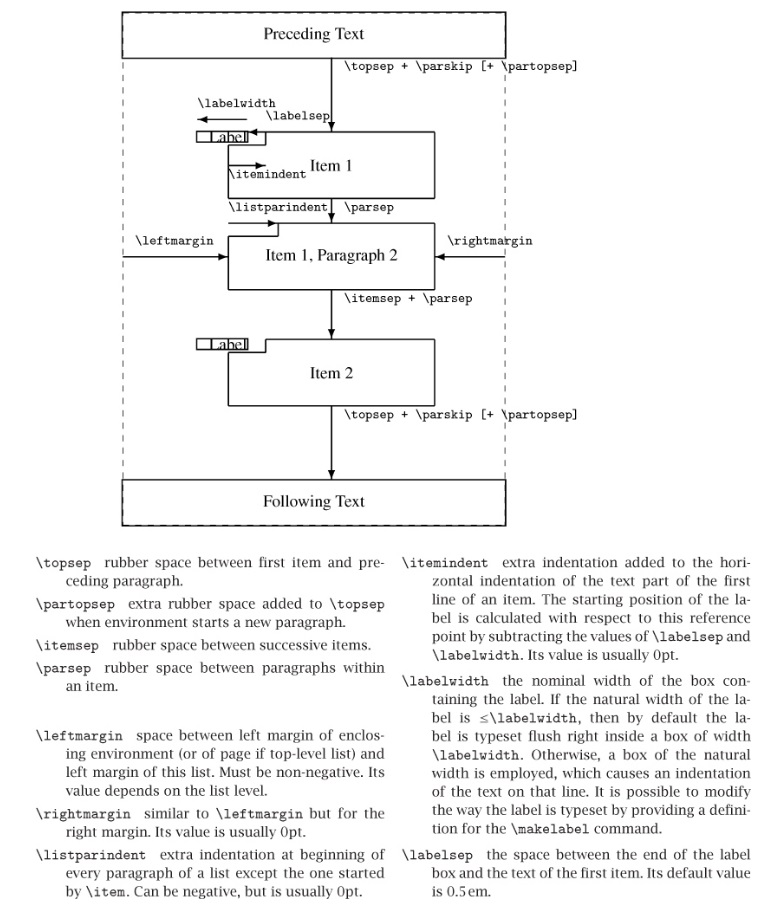
\includegraphics[width=\linewidth]{fig/1.jpg}
        \caption{enumerate 设置}
        \label{fig:1}
    \end{figure}

    \begin{enumerate}\setcounter{enumi}{\value{tmp}}
        \item 抄录和代码环境.\footnote{\lstinline|\\verb| 似乎不能在脚注中使用, 不过能用 \lstinline|\\lstinline| 代替.} \par \verb"\int", \verb*|\int main|, 以及 \verb!verbatim! 环境. 更复杂的, 可以参考 \verb|fancyvrb| 宏包.
        \item 代码高亮. 行内代码 \lstinline|int main()|, 多行代码
        \begin{lstlisting}[language=C]
#include<iostream>
int main()
{
    cout<<"hello world!"; //xeCJK已经支持中文,不必再转义.
    return 0;
}
        \end{lstlisting}
        \item \verb|tabbing| 环境.
        {\itshape\begin{tabbing}
            \bfseries 项目 \phantom{手掌上受力点到手腕的距离} 取值\=\\
            手臂质量 \> $m=$\'$0.2602925$\\
            手掌上受力点到手腕的距离 \> $L_p=$\'$0.090$ \\
            上臂长度 \> $L_1=$\'$0.30$ 
        \end{tabbing}}\par 
        有一点复杂. 制表位记录一个位置, 并不意味着添加一个制表符. 如果要排版复杂的伪代码, 使用 \verb|algorithm2e| 宏包.
        \item 脚注.
        \begin{enumerate}
            \item 在不能使用脚注的地方, 可以采用\autoref{tab:mathfonts} 中的方法. 其中, \verb|\footnotemark[<数字>]| 在没有可选参数时使脚注计数器自增.
            \item 脚注的脆弱命令. 在章节或图表标题中使用脚注, 应当用 \verb|\protect\footnote|. 
            \item \setcounter{tmp}{\value{footnote}}{ \renewcommand{\thefootnote}{\fnsymbol{footnote}}\setcounter{footnote}{1} 可能遇到符号标注的脚注\footnote{text}. \par 如果节标题中有脚注, 应当避免出现在目录中. \par
                \verb|\section[标题]{标题\protect\footnote{脚注}}|\par \uline{\fangsong 注}: \verb|\renewcommand| 是有作用域的, 为当前域及子域.
            }
            \setcounter{footnote}{\value{tmp}}
        \end{enumerate}
        \item 边注. \marginpar[有一说一]{很少使用.} 
        \item 使用 \verb|\appendix| 命令, 改变此后的文档结构编号为字母, 标志着附录开始. 
        \item 控制标题格式, 使用 \texttt{titlesec} 宏包, 请查阅文档. 
        \item 交叉引用.
        \begin{enumerate}
            \item 常用标签前缀
            \begin{multicols}{2}
                \begin{itemize}
                    \item \verb|part|: part
                    \item \verb|chap|: chapter
                    \item \verb|sec|: section
                    \item \verb|subsec|: subsection
                    \item \verb|subsubsec|: subsubsection
                    \item \verb|para|: paragraph
                    \item \verb|subpara|: subparagraph
                    \item \verb|fig|: figure
                    \item \verb|tab|: table
                    \item \verb|eq|: equation
                    \item \verb|fn|: footnote
                    \item \verb|thm|: theorem
                    \item \verb|algo|: algorithm
                \end{itemize}
            \end{multicols}
            \item 引用命令
            \begin{itemize}
                \item {\LaTeX} 定义: \verb|\ref| 和 \verb|\pageref|. \par
                \emph{第 \pageref{sec:1st} 页中的第 \ref{sec:1st} 章描述了一些在 {\LaTeX} 中处理普通文本的方法. }
                \item \texttt{amsmath} 定义: \verb|\eqref|, 自动为公式引用加括号. \par \emph{ 式 \eqref{eq:1st} 是勾股定理. }
                \item \texttt{hyperref} 定义: \verb|\autoref|, 自动为引用的数字添加前缀. 这个前缀由 \verb|\某autorefname| 定义, 默认已定义为英文. 修改方法: \verb|\renewcommand{\figureautorefname}{图}|. 
                \item \texttt{nameref} 定义: \verb|\nameref|, 获得被引对象的标题. 
                \par \emph{\autoref{tab:1} 是\nameref{tab:1}. }
            \end{itemize}
        \item \texttt{hyperref} 会使得文章中所有的交叉引用成为超链接. 
        \item \texttt{hyperref} 提供 \verb|\url{URL}|、\verb|\href{URL}{text}|、\verb|\path{filepath}| 以及 \verb|\hyperref[label]{text}|. 它还提供 \verb|\hypertarget{name}{text}| 和 \verb|\hyperlink{name}{text}|, 将一个地方的文字连接到另一个地方. 
        \item \texttt{hyperlink} 提供了一些有关 pdf 书签的命令. 例如自定义书签 \verb|\pdfbookmark[level]{text}{name}|, 额外定义书签中的显示名以防止难看的书签 \verb|\texorpdfstring{text}{PDFstring}|.
        \end{enumerate}
    \end{enumerate}


    \section{数学排版}
    \begin{enumerate}
        \item 行内公式的形式: \verb|$...$|\footnote{错误检查不如后两者, 但由于形式简单而广受喜爱.}, \verb|\(...\)|, \verb|\begin{math}...\end{math}|. 
        \item \begin{theorem}[勾股定理]
            勾三股四玄五
        \end{theorem}\begin{equation}\label{eq:1st}
            AB^2+BC^2=AC^2
        \end{equation}
        \begin{inference}[勾股定理的另一种形式]
            玄五股四勾三
        \end{inference}
        \item 独行公式后如果有标点, 应当放在数学环境内部.
        \item 数学公式中的撇号 $'$ 是一种特殊的上标. 实际上, $\verb|'|\cong\verb|^\prime|$. 
        \item 由 \texttt{galois} 提供的一个特殊符号: 复合函数 $h=f\comp g$.
        \item 要在符号的左边加角标, 最好\footnote{另一种方法是给前面的空分组加上下标, 但是得到的间距和对齐不合理.}使用 \texttt{mathtools} 宏包提供的 \verb|\prescript{NW}{SW}{content}|.\par \emph{$\prescript{227}{90}{\mathrm{T\/h}}^{+}$ 是一个例子\footnote{我不知道化学式是否要连字, 但是 ``Th'' 是一个少见连字, 此处分开总没有错.}, 但是排版化学式最好使用 \texttt{mhchem} 宏包. } \par
        然而, 如果要给巨算符左侧添加角标, 应当使用 \verb|\sideset{left}{right}{symbol}|. \par
        \begin{equation}
        \sideset{_a^b}{_c^d}{\sum}_{i=1}^{n} i^2=\frac{n(n+1)(2n+1)}{6}
        \end{equation}  
        \item 如果要让方程式按节编号, 可以重定义其计数器. {\CJKsetecglue{}\ttfamily\textbackslash numberwithin\{$\langle\text{计数器}_1\rangle$\}\{$\langle\text{计数器}_2\rangle$\}} 是在 \texttt{amsmath} 中定义的命令, 扩展了 \texttt{newcounter} 的自动清零功能并定义其编号格式.  \numberwithin{equation}{section} %page101
        \begin{equation}
        AB^2+BC^2=AC^2
        \end{equation}
        \item 数学堆叠符号
        \begin{itemize}
            \item 上下标记 \verb|\overset{marks}{text}|, \verb|\underset|. 
            \item 上下横线 \verb|\overline{text}|, \verb|\underline|. 
            \item 上下箭头 \verb|\overleftarrow{text}|, \verb|\overrightarrow|, \verb|\overleftrightarrow|...
            \item 上下花括弧 \verb|\overbrace{text}^{expr}|, \verb|$\underbrace$|.
            \item \texttt{mathtools} 提供了上下方括弧 \verb|\overbracket[width][height]{text}|, \verb|\underbracket|\footnote{我也不晓得怎么回事, 但是这默认线宽就太离谱了.}. 
            \begin{equation}
            \overline{a+b}=\underbrace{a_1+a_2+\cdots a_n}_{\text{共} n \text{项}} + \norm{\overrightarrow{AB}} + \underbracket[.8pt]{\overbracket{1+2}+3}_6 
            \end{equation}
        \end{itemize}
        \item 连分式 \verb|\cfrac[align(lcr)]{numerator}{denominator}|.
        \begin{equation}
        \bdint{x}{0}{\infty}{\ue^{-x^2}}=\frac{\sqrt{\pi}}{2}-\cfrac{\ue^{-a^2}}{2a+\cfrac{1}{a+\cfrac{2}{2a+\cfrac{3}{a+\cfrac{4}{2a+\cdots}}}}}
        \end{equation}
        \item 行内的分式有时仍过分拥挤, 可以写为 $a/b$. 然而 $1/a+b$ 可能引入歧义, 可用 \texttt{xfrac} 宏包的 \verb|\sfrac{}{}| 来获得合适的短小分式, 如 $\sfrac1a+b$.
        \item 类似的, 二项式系数 \verb|\binom{above}{below}|. \begin{equation}
        (a+b)^2=\binom20a^2+\binom21ab+\binom22b^2
        \end{equation}
        \item 根号会随字母的高度和深度变化而变化, 如 $\sqrt a$, $\sqrt y$. 此时, 可以使用 \verb|\mathstrut| 获得一个有一个圆括弧高度和深度的框架, 效果为 $\sqrt{\mathstrut a}$, $\sqrt{\mathstrut y}$.
        \item 矩阵. \par 
        \begin{equation}
        \begin{matrix}
        a & b\\c & d
        \end{matrix}= 
        \begin{pmatrix}
        a & b\\c & d
        \end{pmatrix}=
        \begin{bmatrix}
        a & b\\c & d
        \end{bmatrix}=
        \begin{Bmatrix}
        a & b\\c & d
        \end{Bmatrix}=
        \begin{vmatrix}
        a & b\\c & d
        \end{vmatrix}=
        \begin{Vmatrix}
        a & b\\c & d
        \end{Vmatrix}
        \end{equation}
        上面的环境都有对应的带星号宏包, 可以指定列对齐方式. 
        \begin{equation}
        \begin{pmatrix*}[r]
        10 & -10 \\ -20 & 3
        \end{pmatrix*}
        \end{equation}
        矩阵中常用省略号
        \begin{equation}
        A=\begin{bmatrix}
        a_{11} & \cdots & a_{1n} \\
        & \ddots & \vdots \\
        && a_{nn}
        \end{bmatrix}
        \end{equation}
        
        行内, 可以使用小矩阵 $\left(\begin{smallmatrix}
        a&b\\c&d
        \end{smallmatrix}\right) $
        \item 如果要在巨算符的上下标中加入多行, 可以使用 \verb|\substack| 或者 \verb|subarray| (可以指定对齐方式 \verb|lcr|).
        \begin{equation}
            \sum_{\substack{0<i<n \\ 0<j<i}} A_{ij}=\sum_{\begin{subarray}{l}
                i<10 \\ j<100 \\ k<1000
                \end{subarray}} X(i,j,k)
        \end{equation}
        \item 数学公式中, 只有变量使用默认的意大利体, 而常数 $\ue$、圆周率 $\upi$ 以及虚数单位 $\ui$ 均应使用直立体.
        \item 一些数学字体, 见表 \ref{tab:mathfonts}. 
        \begin{table}[htb]
            \centering
            \caption{标准 \LaTeX\ 及宏包提供的数学字体}
            \label{tab:mathfonts}
            \begin{tabular}{lll}
                \toprule
                类别 & 字体命令 & 输出效果 \\
                \midrule
                数学环境的默认字体 & \verb|\mathnormal| & $\mathnormal{ABCHIJXYZabchijxyz12345}$ \\
                意大利体 & \verb|\mathit| & $\mathit{ABCHIJXYZabchijxyz12345}$ \\
                罗马体 & \verb|\mathrm| & $\mathrm{ABCHIJXYZabchijxyz12345}$ \\
                粗体 & \verb|\mathbf| & $\mathbf{ABCHIJXYZabchijxyz12345}$ \\
                无衬线体 & \verb|\mathsf| & $\mathsf{ABCHIJXYZabchijxyz12345}$ \\
                打字机体 & \verb|\mathtt| & $\mathtt{ABCHIJXYZabchijxyz12345}$ \\
                花体\footnotemark & \verb|\mathcal| & $\mathcal{ABCHIJXYZabchijxyz12345}$\\
                数学粗体 (\verb|bm|) & \verb|\bm| & $\bm{ABCHIJXYZabchijxyz12345}$ \\
                黑板粗体 (\verb|amssymb|) & \verb|\mathbb| & $\mathbb{ABCHIJXYZabchijxyz12345}$ \\
                花体 (\verb|mathrsfs|) & \verb|\mathscr| &$\mathscr{ABCHIJXYZabchijxyz12345}$\\
                \bottomrule
            \end{tabular}
        \end{table}\par
        \emph{空集 $\varnothing$ 的基数是 $0$, 自然数集 $\mathbb{N}=\{1,2,3,\ldots\}$ 的基数是 $\aleph_0$, 则实数集 $\mathbb{R}$ 的基数 $\#\mathbb{R}=\aleph_1=2^{\aleph_0}$. }
        \item 容易忽视的数学普通符号: $\imath$ 和 $\jmath$ 用于加重音, $\ell$ 用于区分 $l$ 和 $1$.
        \item \footnotetext{只支持大写字母. 一些专业字体包可以让其支持小写.}使用 \verb|\DeclareMathOperator| 来定义新的数学算子, 使用 \verb|\operatorname| 来临时使用自定义的数学算子. \begin{equation}
        \Var(X)=\expect(X-\mu)^2
        \end{equation}
        \item 取模和同余的符号有一组命令.
        \begin{align}
        r&=m\bmod n &  &\text{\lstinline|r = m \\bmod n|} \notag\\
        x&\equiv y \pmod b & &\text{\lstinline|x\\equiv y \\pmod b|}\notag\\
        x&\equiv y \mod c & &\text{\lstinline|x\\equiv y \\mod c|}\notag\\
        x&\equiv y \pod c & &\text{\lstinline|x\\equiv y \\pod c|}
        \end{align}
        \item 数学环境中的冒号是二元关系符号, 两侧间距相等, 可以用来代替比例运算符号, 但是更准确的是使用 \verb|\mathbin|. 要使用数学标点, 使用 \verb|\colon| (相当于 \verb|\mathpunct{:}|).
        \begin{align}
        f(x)&:=x^2 & 4\mathbin{:}2&=2\mathbin{:}1 & f&\colon x\mapsto x^2
        \end{align}
        \item 当二元关系符没有自带的否定符号时, 在前面加 \verb|\not| 得到否定形式. 
        \item \texttt{amsmath} 和 \texttt{extarrows} 提供了变长箭头等符号, 可以在上下方添加说明.
        \begin{equation}
        \mu\xlongequal{\text{def}}\expect X
        \end{equation}
        \item \LaTeX\ 和 \texttt{amsmath} 定义了几个逻辑符号命令: \verb|\iff|, \verb|\implies|, \verb|\impliedby|, \verb|\And|. 符号与一般相同, 而间距比一般的运算符和关系符要大.
        \begin{align}
        x=y &\implies x+a=y+a \notag\\
        x=y &\impliedby x+a=y+a \notag\\
        x=y &\iff x\leqslant y \And x\geqslant y 
        \end{align}
        \item 命令 \verb|\mathbin| 和 \verb|\mathrel| 可创造二元运算符和二元关系符.
        \item 左右定界符的前后间距不同. 使用命令 \verb|\mathopen| 和 \verb|\mathclose| 可以声明新的定界符. 
        \item 可变大小的定界符.
        \begin{enumerate}
            \item 使用 \verb|\left|, \verb|\right| 和 \verb|\middle| 来自动调整.
            \begin{equation}
            \Pr\left(X>\frac12\middle\vert Y=0\right)=\left.\int_0^1 p(t)\dif{t}\middle/ (N^2+1)\right.
            \end{equation}
            \item 使用 \verb|\big|, \verb|\Big|, \verb|\bigg|, \verb|\Bigg| 以及各自对应的 \verb|-l|, \verb|-r|, \verb|-m| 命令.
            \begin{equation}
            1+\Bigl( 2-\bigl( 3\times(4\div5) \bigr) \Bigr)
            \end{equation}
        \end{enumerate}
        \item 数学省略号 \verb|\ldots| 和 \verb|\cdots|, 大体原则是与前后符号的高度一致. 
        \begin{enumerate}
            \item \texttt{amsmath} 提供的 \verb|\dots| 可以自动识别各种情形.
            \begin{align}
            (1,&\dots,n) & 1+&\dots+n & a=&\dots=z
            \end{align}
            \item 更精细地, \texttt{amsmath} 分别为 comma, binary, multiplication, integral 和 others 提供了 \verb|\dotsc|, \verb|\dotsb|, \verb|\dotsm|, \verb|\dotsi| 和 \verb|\dotso|.
            \begin{equation}
                \prod_{i=1}^{n} a_i=a_1\dotsm a_n \qquad \int_{0}^{1}\dotsi\int_0^1
            \end{equation}
        \end{enumerate}
        \item 多行数学环境.
        \begin{multicols}{2}
            \begin{gather}
            a+b=b+a \\ a\times b=b\times s
            \end{gather}
            \begin{align}
            x&=t+\cos t+1\\
            y&=2\sin t
            \end{align}
            \begin{align*}
            x&=t & x&=\cos t & x&=t \\
            y&=2t & y&=\sin(t+1) & y&=\sin t
            \end{align*}
            \begin{flalign}
            x&=t & x&=2 \\ y&=2t & y&=4
            \end{flalign}
            \begin{alignat}{2} %使用上仿佛是两列一组, 而之间不会自动加间隔
            x&=\sin t &\quad &\text{水平方向} \\
            y&=\cot t & &\text{竖直方向}
            \end{alignat}
            \begin{align}
            x^2+2x&=-1 
            \intertext{移项得} 
            x^2+2x+1&=0
            \end{align}
            \begin{align}
            x^2+2x&=-1 
            \shortintertext{移项得} %间距更小, 由 mathtools 提供.
            x^2+2x+1&=0
            \end{align}
            \begin{subequations}
                \begin{gather}
                    a+b=50\\2a+4b=124
                \end{gather}
            \end{subequations}
        \end{multicols}
        \item 拆分公式
        \begin{multicols}{2}
            \begin{multline} %equation 的分行版本, 首行左对齐, 末行右对齐, 中间居中.
                a+b+c\\
                +d+e+f\\
                +g+h+i\\
                +j+k+l
            \end{multline}
            
            \begin{equation}
            \begin{split}
            &\mathrel{\phantom{=}}(a+b)(a^2-ab+b^2) \\
            &=a^3+b^3
            \end{split}
            \end{equation}
            \begin{equation}
            \begin{split}
            % 另一种实现
            &(a+b)(a^2-ab+b^2) \\
            ={}&a^3+b^3
            \end{split}
            \end{equation}
            
%            \begin{dmath} % breqn 提供的自动换行. 其内上下标必须使用分组. 在这里使用似乎有 bug, 把所有的减号显示为某种加号.
%                \frac12(\sin(x+y)+\sin(x-y))=\frac12(\sin x\cos y+\cos x\sin y)+\frac12(\sin x\cos y - \cos x\sin y)=\sin x\cos y
%            \end{dmath}
            
        \end{multicols}
        \item \verb|cases| 与 \verb|dcases| 环境.
        
        \begin{minipage}[c][5em]{0.49\linewidth}
            \begin{equation}
            D(x)=\begin{cases}
            1, & x\in\mathbb{Q} \\ 0, & x\notin\mathbb{Q}
            \end{cases}
            \end{equation}
        \end{minipage}\makebox[0.01\linewidth][r]{\rule[-2.2em]{0.4pt}{5em}}        \begin{minipage}[c][5em]{0.5\linewidth}        
            \begin{equation}
            \abs{x-\frac12}=\begin{dcases}
            x-\frac12, & x\geqslant \frac12 \\ \frac12-x, &x<\frac12
            \end{dcases}
            \end{equation}
        \end{minipage}
        \item 组合公式块可以使用对应的 \verb|gathered|, \verb|lgathered|, \verb|rgathered|, \verb|aligned|, \verb|alignedat| 和 \verb|multlined| 来得到. 
        \begin{equation}
        \begin{aligned}
        x+y&=-1 \\ x+y+z&=2 \\ xyz&=-6
        \end{aligned} \implies 
        \begin{aligned}
        x+y&=-1 \\ xy&=-2 \\ z&=3 
        \end{aligned} \implies 
        \begin{alignedat}{3}
        x&=1, &\quad y&=-2, &\quad z&=3 \\ 
        \text{或} x&=-2, & y&=1, & z&=3
        \end{alignedat}
        \end{equation}
        
        \uline{\fangsong 注}: 可以在 \verb|align| 或 \verb|split| 等中的其中一行使用 \verb|multlined| (带可选参数 \verb|[t]|), 得到较好的折行效果.
        \item 数学公式的字号受外面的文本字号控制. 如果要在公式内部调整字号, 就需要来回切换. 
        \begin{equation}
        \mathop{\text{\Large$\D\sum_i$}}\dfrac{\D\int f_i(x)\dif x}{\D\oint g_i(x)\dif x}
        \end{equation}
        \item 行内公式只允许在二元关系符和二元运算符后断行. 在省略乘号的连乘式中, 可以用 \verb|\*| 来提示可能的断行点. \par  
        \fbox{\parbox{5em}{$f(x)\*g(x)\*h(x)$}}
        \item 使用数学间距来微调, 例如
        \begin{align}
            &\text{调整前} &&\sqrt2x && \sqrt{\log x} && x^2/2 && \vert{\gets}5{\to}\vert \\
            &\text{调整后} &&\sqrt2\,x && \sqrt{\,\log x} && x^2\!/2 && \vert\!{\gets}5{\to}\!\vert 
        \end{align}
    \end{enumerate}


    \section{绘制图表}
    \begin{enumerate}
        \item 表 \ref{tab:1} 是一个表格的例子.
        \begin{table}[htb]
            \centering
            \caption{一个表格的例子}
            \label{tab:1}
            \begin{tabular}{|c|*{2}{S|}}%'S' provided by siunitx, along with 's' for units.
                \hline \bfseries 姓名 & \multicolumn{1}{c|}{\bfseries 支出 1} & \multicolumn{1}{c|}{支出 2} \\
                \hline 张三 & 21.2e5 & 2.655 \\
                \hline 李四 & 2.5 & 3\\
                \hline
            \end{tabular}
        \end{table}
		\item 多栏文档中, 可以用 \texttt{figure*} 等环境得到跨栏浮动体, 位置只能是 \texttt{tp}. 
		\item 最宽松的浮动体位置是 \texttt{!htbp}, 其中 \texttt{!} 用来忽略一页中数量和占用大小的限制. 使用 \texttt{H} (由 \texttt{float} 宏包提供) 可以取消其浮动性. 
        \item 表格的列格式说明符:
        \begin{itemize}
            \item \texttt{lrc|}: 常见的对齐单元格与竖线
            \item \verb|p{width}|: 固定列宽, 并自动换行. 默认左对齐, 使用 \verb|\centering| 等命令可改变. 
            \item \verb|@{text}|: 添加任意内容. 该内容没有列间距, 在表格内容定义中不出现.
            \item \verb|*{count}{char}|: 简写, 重复多次.
            \item (以下为 \texttt{array} 宏包提供) \verb|m{width}|: 类似 \verb|p|, 垂直方向居中对齐.
            \item \verb|b{width}|: 类似 \verb|p|, 垂直方向上与底行对齐.
            \item \verb|<{text}|: 把内容插入前一列的末尾.
            \item \verb|>{text}|: 把内容插入后一列的开头. \footnote{这两个命令常用于设定一整列的格式}
            \item \verb|!{text}|: 把内容作为表格线处理, 相比 \verb|@| 保留左右间距.
        \end{itemize}
        \item \verb|@{}| 可以用来消除列间距, 例如 $\left[\begin{tabular}{@{}c@{}}
        \text{文本} \\ \text{数学}
        \end{tabular}\right]$ (习惯上, 矩阵左右列外侧的间距总是被消除); 还可以在其中使用 \verb|\extracolsep{sep}| 来增加它及它之后所有列左侧的间距 (但本列的间距会被消除).
        \item \texttt{array} 宏包提供了 \verb|\newcolumntype{name}{argument}| 来定义新的列格式说明符, 简化列格式说明区, 易于辨认. \par \verb|\newcolumntype{P}[1]{>{\setlength\parindent{2em}}p{#1}}|
        \item 表格单元的合并与分割.
        \begin{itemize}
            \item 合并同行单元格命令 \verb=\multicolumn{cols}{|l/c/r/p/@|}{content}=, 它会消除表格列后的竖线 (如果是第一列, 也会消除左侧的). 也用于改变单元格格式.
            \item \texttt{multirow} 提供了合并同列单元格命令 \verb=\multirow{rows}{width}{content}= 或\\ \verb|\multirow{rows}*{content}|. 第一种形式能自动换行, 第二种形式自动确定宽度.
            \item 使用嵌套的表格可以拆分单元格. 应在表格两侧使用 \verb|@{}| 来多余的间距和竖线. 
            \item {\color{gray} \verb|\cline{i-j}| 可以在表格中画一段不完整的表格线, 可以用来产生跨行单元格的效果.}
            \item {\color{gray} \verb|\vline| 可以在单元格中画一条只占一行高度的竖线, 可以用来拆分单元格 (要注意加上适当的间距, 准确地讲是 \verb|\tabcolsep|). }
        \end{itemize}
        \item \texttt{makecell} 宏包提供的 \verb|\makecell| 命令使得能够\begin{tabular}[t]{@{}c@{}}
            \makecell[rt]{在单元格中\\自由换行.} %两个表格同时设置 [t] 选项才能得到顶端对齐效果.
        \end{tabular}
        \par 类似地, \texttt{makecell} 还提供了 \verb|\thead| 命令, 产生 \begin{tabular}{@{}c@{}}
            \thead{字体较小\\上下间距较大}
        \end{tabular}的单元格, 更适合文字较多的表头. 
        \item 同时使用 \texttt{multirow} 和 \texttt{makecell} 时, 有命令 \verb|multirowcell| 和 \verb|mutlirowthead|, 可以在跨行单元格中随意换行.
        \item 如要对表头进行斜线分割, 可以使用 \texttt{diagbox} 宏包的 \verb|\diagbox[options]{left}{right}| 和 \verb|\diagbox[options]{left}{mid}{right}| 命令. 
        \item \autoref{tab:complextable} 是\nameref{tab:complextable}.
        
        \begin{table}[htb]
            \centering
            \caption{一个复杂表格的例子}
            \label{tab:complextable}
            \begin{tabular}{|c|c|c|S|S|S|S|S|}
                \hline 
                \multirowcell{2}{摩擦副\\配对材料} & \multicolumn{2}{c|}{\multirow{2}*{\diagbox[height=2\normalbaselineskip]{锁紧结构}{锁紧力矩\\[-1ex]\si{\N\cdot\m}}}} & \multicolumn{5}{c|}{供油压力 (\si{\MPa})} \\
                \cline{4-8} & \multicolumn{1}{c}{} & & \multicolumn{1}{c|}{$2$} & \multicolumn{1}{c|}{$5$} & \multicolumn{1}{c|}{$7$} & \multicolumn{1}{c|}{$10$} & \multicolumn{1}{c|}{$12$} \\
                \hline \multirow{5}*{调质钢} & \multirowcell{5}{摩\\擦\\锥} & $\theta=\ang{60}$, 单槽 & 1.3 & 2.6 & 2.9 & 3.5 & 3.8 \\
                \cline{3-8} & & $\theta=\ang{60}$, 双槽 & 1.8 & 3.4 & 3.7 & 4.5 & 5.2 \\
                \cline{3-8} & & $\theta=\ang{64}$, 双槽 & 1.2 & 2.6 & 2.9 & 3.4 & 3.7 \\
                \cline{3-8} & & $\theta=\ang{36}$, 双槽 & 1.5 & 3.3 & 4.3 & 4.4 & 4.6 \\
                \cline{3-8} & & $\theta=\ang{20}$, 双槽 & 1.6 & 3.3 & 3.8 & 5.0 & 5.5 \\
                \hline \multirow{2}*{H62} & \multicolumn{2}{c|}{内摩擦环} & 1.6 & 2.9 & 4.0 & 4.6 & 5.1 \\
                \cline{2-8} & \multicolumn{2}{c|}{外摩擦环} & 7.6 & 8.6 & 9.5 & 10.5 & 11.7 \\
                \hline
            \end{tabular}
        \end{table}
        \item \verb|\includegraphics| 命令中的 \texttt{height} 参数仅仅指图片的高度. 图片旋转后可能出现深度, 因此应当使用 \texttt{totalheight}.
        \item \texttt{graphicx} 提供了一些 (针对盒子的) 几何变换命令.
        \begin{itemize}
            \item \verb|\scalebox{h-scale}[v-scale]{text}| 按\scalebox{0.5}{比例}\scalebox{0.5}[1]{放}\scalebox{0.5}[1]{缩}. 
            \item \verb|\reflectbox{text}| 用来做\reflectbox{镜像}反射.
            \item \verb|\resizebox{h-length}{v-length}{text}| 放缩内容到指定宽高. 其中一个尺寸可以设置为叹号 \texttt{!} 来表示随另一个量放缩. 
            \item \verb|\rotatebox[options]{angle}{text}| 逆时针旋转内容. 选项可以设置 \verb|origin| 和 \verb|units|.
        \end{itemize}
        \item 使用 \verb|pdflscape| 宏包提供的 \verb|landscape| 环境来得到旋转的页面. 如果仅仅只是需要一个旋转的浮动环境, 可以使用 \verb|rotfloat| 宏包, 它为所有浮动环境提供了一个 \verb|sideways| 打头的旋转环境. 
        \item \texttt{caption} 宏包提供了标题控制, 这篇样例中已经进行了自定义. 详见《入门》\emph{Page 340--349}.
        \item \texttt{subcaption} 宏包提供的 \verb|subfigure| 和 \verb|subtable| 环境, 可以放置子图表并自动使用子标题. 图 \ref{fig:2} 是一个并排子图的例子. 引用时, \verb|\ref| 得到 \ref{fig:2/a}, \verb|\subref| 得到 \subref{fig:2/a}.
        \begin{figure}[htbp]
            \centering
            \begin{subfigure}[b]{0.27\textwidth}
                \centering
                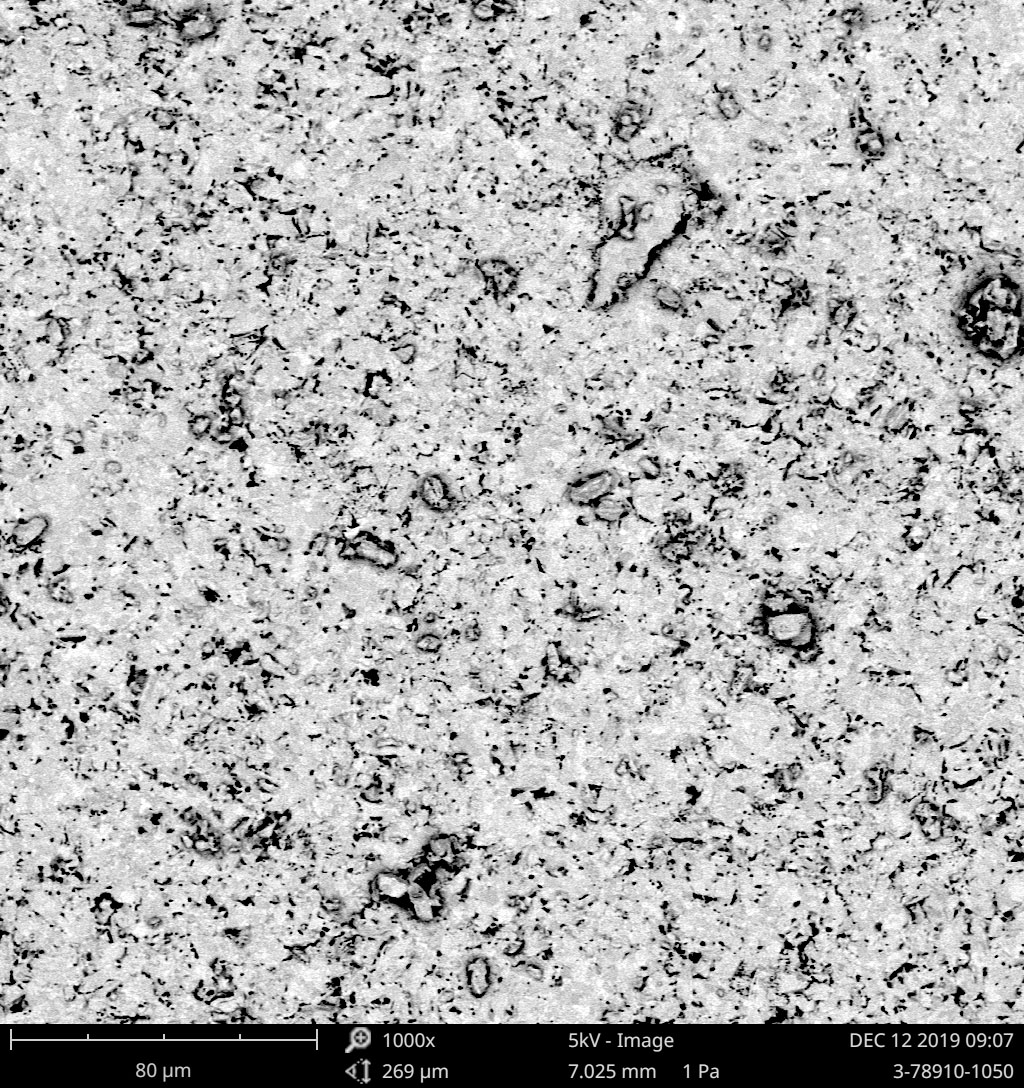
\includegraphics[width=0.9\linewidth]{fig/3-78910-10500001.jpg}
                \caption{\SI{1050}{\celsius}, $1000\text{X}$}
                \label{fig:2/a}
            \end{subfigure}
            \begin{subfigure}[b]{0.27\textwidth}
                \centering
                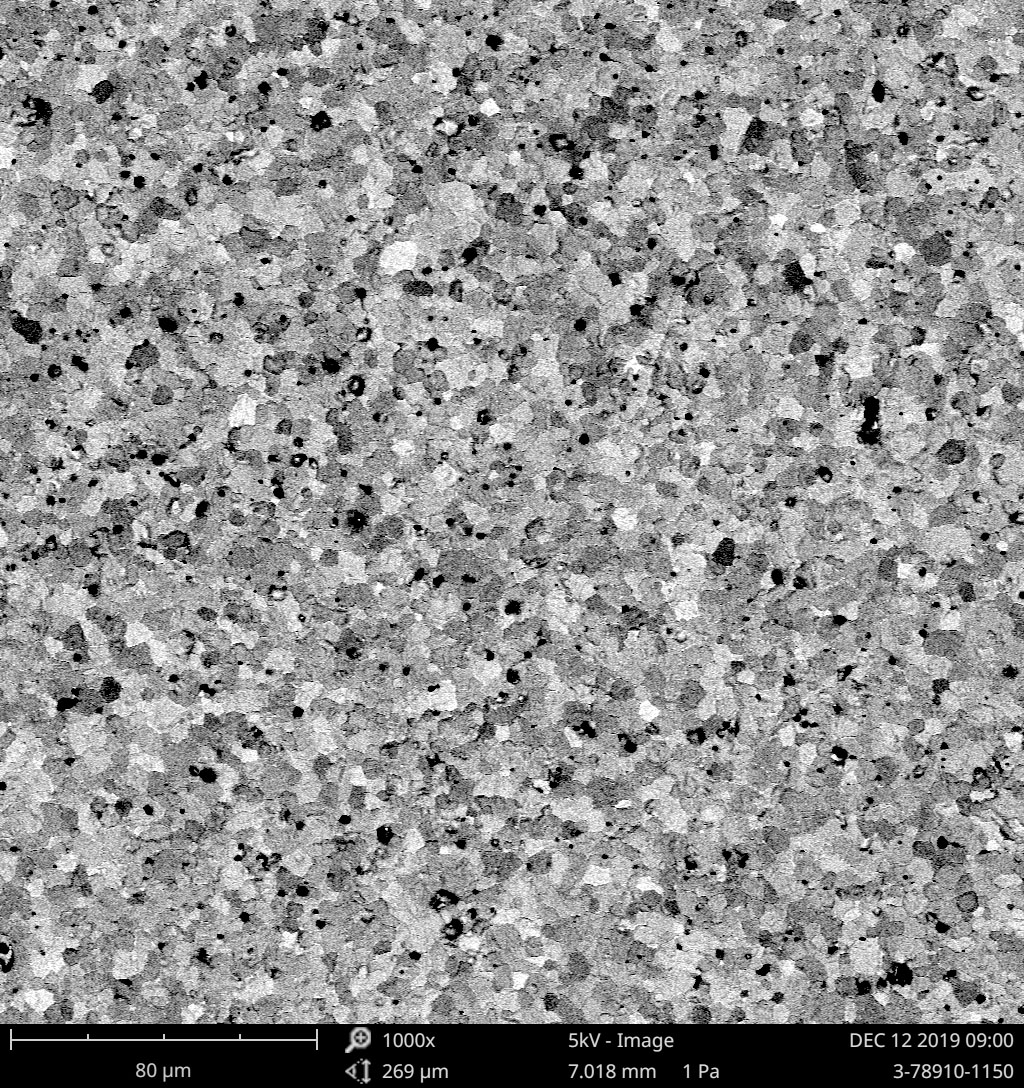
\includegraphics[width=0.9\linewidth]{fig/3-78910-11500001.jpg}
                \caption{\SI{1150}{\celsius}, $1000\text{X}$}
            \end{subfigure}
            \begin{subfigure}[b]{0.27\textwidth}
                \centering
                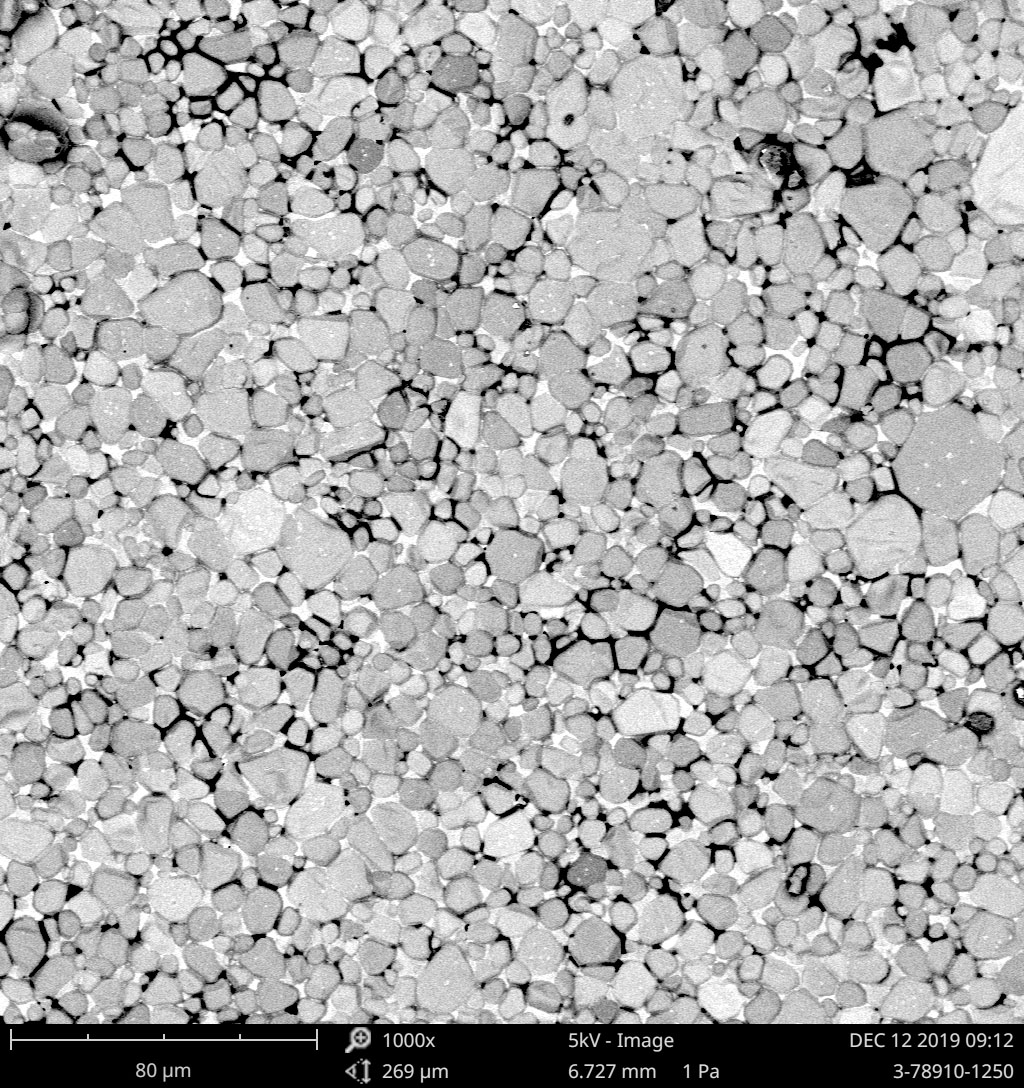
\includegraphics[width=0.9\linewidth]{fig/3-78910-12500001.jpg}
                \caption{\SI{1250}{\celsius}, $1000\text{X}$}
            \end{subfigure}
            \\[10pt]
            \begin{subfigure}[b]{0.27\textwidth}
                \centering
                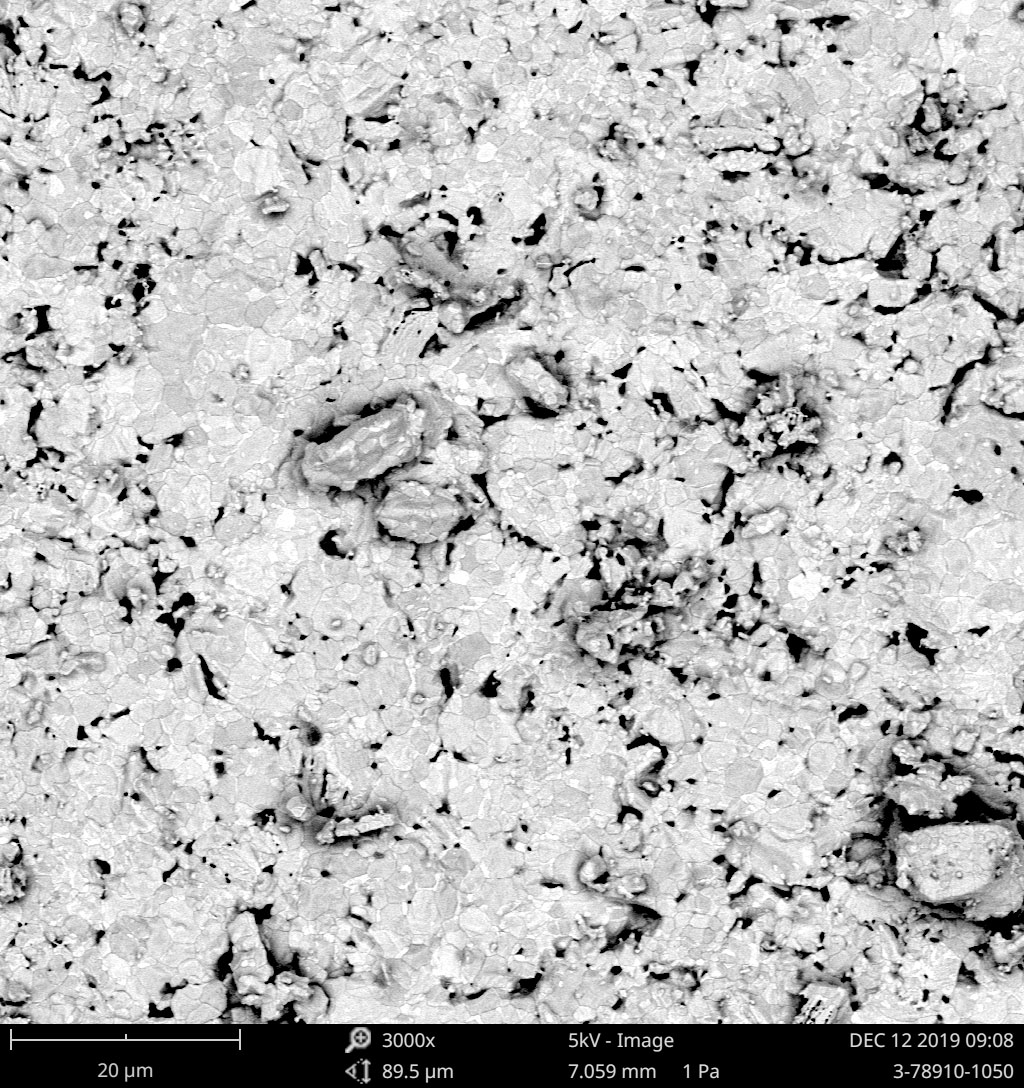
\includegraphics[width=0.9\linewidth]{fig/3-78910-10500002.jpg}
                \caption{\SI{1050}{\celsius}, $3000\text{X}$}
            \end{subfigure}
            \begin{subfigure}[b]{0.27\textwidth}
                \centering
                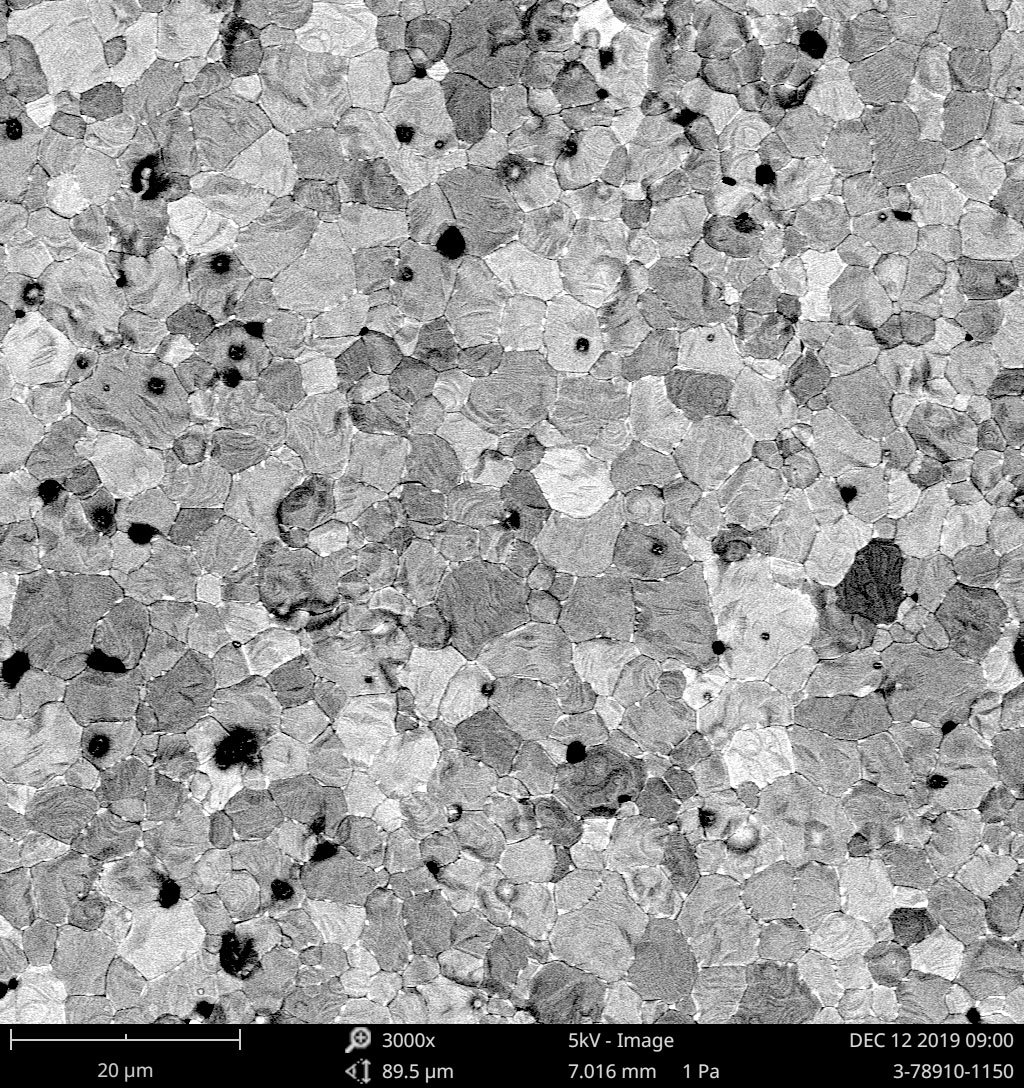
\includegraphics[width=0.9\linewidth]{fig/3-78910-11500002.jpg}
                \caption{\SI{1150}{\celsius}, $3000\text{X}$}
            \end{subfigure}
            \begin{subfigure}[b]{0.27\textwidth}
                \centering
                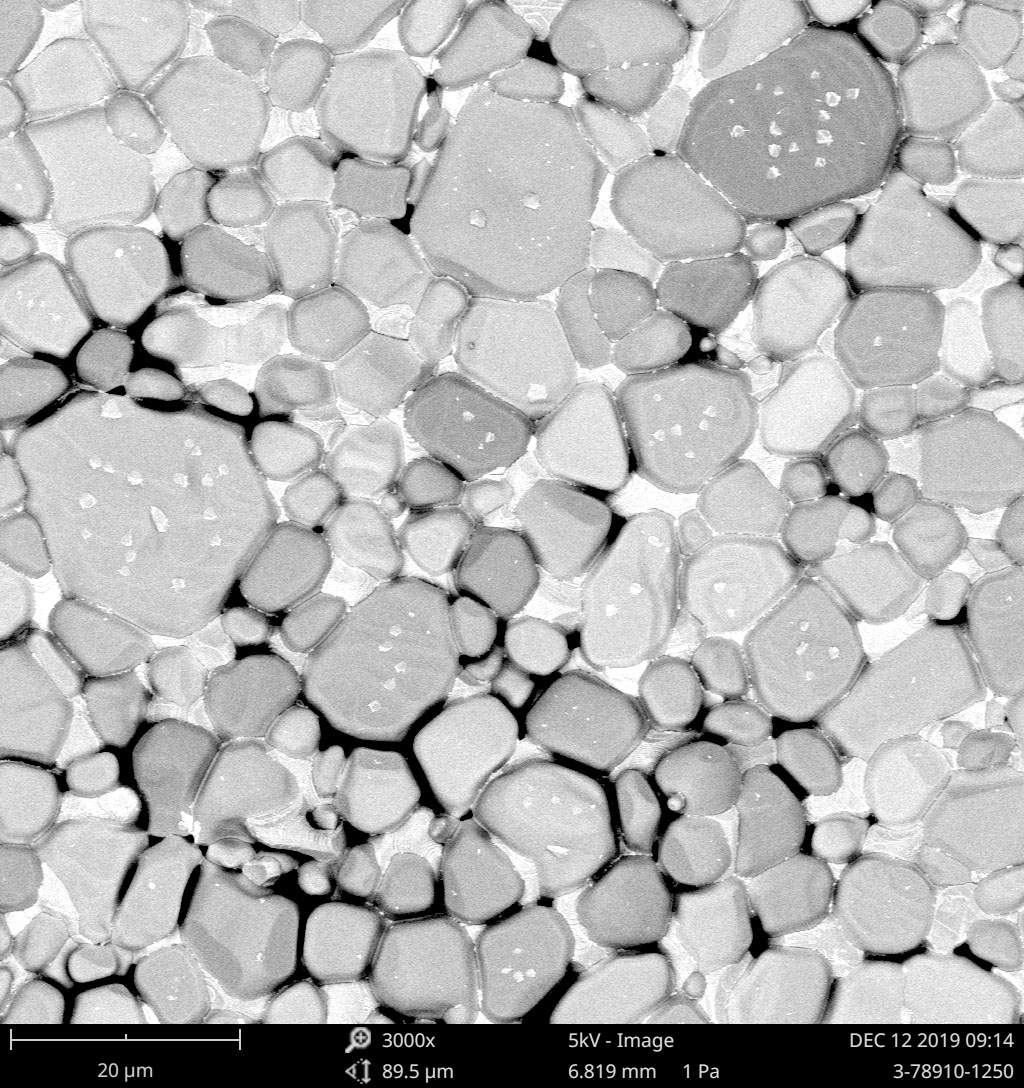
\includegraphics[width=0.9\linewidth]{fig/3-78910-12500002.jpg}
                \caption{\SI{1250}{\celsius}, $3000\text{X}$}
            \end{subfigure}
            \caption{并排子图样例}
            \label{fig:2}
        \end{figure}
        \item {\color{red} \verb|\color| 命令改变此后的所有文字, 而 \verb|\textcolor| 只改变\textcolor{blue}{参数中的文字}.} \verb|\pagecolor| 改变页面背景, \verb|\colorbox| 和 \verb|\fcolorbox| 提供\colorbox{green}{不带边框}和\fcolorbox{brown}{pink}{带边框}的彩色盒子.
        \item 彩色表格由 \texttt{colortbl}实现, 而使用带 \verb|table| 选项的 \texttt{xcolor} 宏包会自动调用 \texttt{colortbl}. 
        \begin{itemize}
            \item 设置表列颜色 \verb|\columncolor[color model]{color}[left overhang][right overhang]|, 使用在 \verb|>{}| 中. 默认的左右外伸参数是 \verb|\tabcolsep|, 以保证文字之外的表列间隙有色彩填充.
            \item 设置表行颜色 \verb|\rowcolor[color model]{color}[left overhang][right overhang]|, 用在一行的开头.\par \verb|\rowcolor| 可能会覆盖用由 \verb|\multirow| 产生的跨行单元格. 解决方法是, 将 \verb|\multirow| 放在最后一行输出, 并向上跨越负数行.
            \item 改变个别单元格的颜色 \verb|\cellcolor[color model]{color}[left overhang][right overhang]|. 
            \item \texttt{xcolor} 宏包扩展了命令 \verb|\rowcolors[commands]{start row}{even row color}{odd row color}|, 可以从起始行开始, 在奇数行和偶数行使用不同的背景色, 同时在前后以及每一行之间执行命令 (可以自动画线)\footnote{这个命令有带星号版本, 只在颜色交错的行之间执行命令}. 命令使用在环境之前. 可见\autoref{tab:colortable} 的例子.
            \begin{table}[htb]
                \centering
                \caption{一个彩色表格的例子}
                \label{tab:colortable}
                \rowcolors{2}{green!20}{green!10}
                \begin{tabular}{crrr}
                    \rowcolor{green!30}
                    项目 & 数值 & 数值 & 数值 \\ 
                    A & 10 & 20 & 30 \\
                    B & 20 & 15 & 40 \\
                    C & 15 & 25 & 37 \\
                    D & 12 & 30 & 42 
                \end{tabular}
            \end{table}
        \end{itemize}
        \item XY-pic 的宏包 \texttt{xy} 用于绘制数学交换图表, 式 \eqref{eq:switch} 是一个例子.
        \begin{equation}\label{eq:switch}
        \begin{gathered}
        \xymatrix@=2ex{
            A'\ar[rd]\ar[rr] & & B'\ar[dd]|\hole\ar[rd] & \\
             & A\ar[rr] & & B\ar[dd] \\
            C'\ar[uu]\ar[rd] & & D'\ar[ll]|\hole\ar[rd] & \\
             & C\ar[uu] & & D\ar[ll] \\
        }
        \end{gathered}
        \end{equation}
        \item Asymptote 是一种类似 C 语法的绘图工具, 内容复杂, \autoref{fig:asymptote} 是一个简单的例子. 可以参考刘海洋等人的教程 \url{https://code.google.com/archive/p/asy4cn/}.
        \begin{figure}[htb]
            \centering 
            \begin{asy}
                real r=0.8cm;
                for (int i=0;i<360;i+=10)
                    draw(circle(dir(i)*r,r));
            \end{asy}
            \caption{Asymptote 一例}
            \label{fig:asymptote}
        \end{figure}
        \item 数学作图可以使用 \texttt{pdfplots} 宏包. 这也是一个内容复杂的宏包, 但是很常用, 附录中给出一些典型的例子, 可以照葫芦画瓢. \par
        \uline{\fangsong 注}: 注释的页码是 pgfplots 的宏包文档 \textit{Manual for Package pgfplots} (2018, Revision 1.16) 的页码. \par
        \uline{\fangsong 注}: pgfplots 有 \verb|\tikzexternalize| 选项, 可以把每一张图放在各自单独的文件中编译, 降低单次编译的资源负担 (编译是有资源限制的, 大量的复杂图像使用的资源总和可能超过这个限制, 编译出错), 提高编译效率. 使用这个技术, 需要在编译命令中加入 \verb|-shell-escape| 选项 (\TeX Live) 或 \verb|-enable-write18| (MiK\TeX).
    \end{enumerate}

    \section{方法和技巧}
    \begin{enumerate}
        \item 使用 \texttt{syntonly} 宏包, 导言区使用命令 \verb|\syntaxonly| 来只检查语法而不编译. 
        \item 在文档类中使用选项 \texttt{draft} 可以着重显示行溢出的盒子. 此时也相当于给 \texttt{graphicx} 提供了 \verb|draft| 选项, 图像将显示为一个带文件名的框. 
        \item \verb|\thepage| 获得当前页码, \texttt{lastpage} 提供的 \verb|\pageref{LastPage}| 可以获得最后一页的页码. \par \emph{page {\thepage} of \pageref{LastPage}}.
        \item \texttt{hyperref} 宏包还提供了一些设置来定义文档的内嵌标题、作者等, 还能定义页面在 pdf 阅读器中的缩放、显示方式、书签等. 参见《\LaTeX\ 入门》第 171 页. 
        \item 制作索引需要 \texttt{makeidx} 宏包. 使用时, 在导言区加入 \verb|\makeindex|, 正文需要索引的关键字加入 \verb|\index{entry}|, 末尾处使用 \verb|\printindex| 打印索引. 索引中的特殊符号 \verb+!|@"+ 各有用途, 其中最后的引号是转义字符. 参见《\LaTeX\ 入门》第 200 页.
        \item 可以使用 \verb|\linebreak[numrange0-4]| 来改变换行行为. 其中 $0$ 表示此处可以换行, $4$ 表示此处必须换行. 换行后, 上一行保持两端对齐. 
        \item 使用 \verb|\leftroot{N}| 和 \verb|\leftroot{N}| 来精调根式开放次数的位置. 如
        \begin{equation}
            \sqrt[n]{\frac{x^2+\sqrt2}{x+y}}=\sqrt[\uproot{16}\leftroot{-2}n]{\frac{x^2+\sqrt2}{x+y}}
        \end{equation}
        \item \verb|\smash| 命令可以忽略内容盒子的高度和深度, 或者加可选参数 \verb|[t]| 和 \verb|[b]| 来只忽略高度和深度. 例如, 可以用来调整根号的高度: $\sqrt{A_{n_k}}$ $\to$ $\sqrt{\smash[b]{A_{n_k}}}$.
        \item 定宽表格和长表格有一系列的宏包和命令, 参见《入门》\emph{Page 297--306}.
        \item 表格虚线可以使用 \texttt{arydshln} 宏包控制, 参见《入门》\emph{Page 311}.
        \item \texttt{graphicx} 提供了命令 \verb|\graphicspath|, 可以指定图像文件的搜索目录, 多个目录用分组隔开. \par \verb|\graphicspath{{pic/}{fig/}}|
    \end{enumerate}

    \section{bdm 与宏包使用偏好}
    \begin{enumerate}
        \item bdm 是一个自定义的宏包, 它的最新版本是 2.0. 由于相对于之前的版本有较大的更新, 且没有向前兼容性, 所以宏包名为 \texttt{bdm2}:\par 
        \verb|\usepackage{bdm2}| \par 
        它提供了下列功能:
        \begin{enumerate}
            \item 简单数学算子: $\rank$, $\image$, $\expect$, $\Var$, $\Cov$, $\Corr$, $\erf$, $\dif\ $.
            \item 带参数的数学算子命令: \verb|\diff[exponent]{var}|, \verb|\patl[exponent]{var}|.
            \item 数学定界符: $\abs{-1}=1$, $\norm{\bmi}=1$.
            \item 数学标记: $\trans{\bmA}$.
            \item 应当使用直立体的数学单位或常量: $\ui$, $\ue$, $\upi$.
            \item 一些长式子的包装简化: \verb|\dfunc[exponent]{numerator}{denominator}|, 以及类似语法的 \verb|\pfunc| (偏微分), \verb|\ddfunc| (显示模式), \verb|\dpfunc|; \verb|\bdint{var}{lower}{upper}{expr}|, \verb|\bdlim{var}{limit}|, \verb|\bdsum{subscript}{superscript}|, \verb|\bdprod{subscript}{superscript}|.
            \item 一些命令的简化: \verb|\bm{*}| $\to$ \verb|\bm*|, 如 $\bma$ 和 $\bmalpha$;\footnote{有一个例外, \lstinline|\\bmO| 的实现是 \lstinline|\\bm{0}|.} \verb|\mr{*}| $\to$ \verb|\mr*|, 如 $\mra$.\footnote{希腊字母的直立体, 请使用 \texttt{upgreek} 宏包提供的 \lstinline|\\up*|}
            \item 大小写罗马数字 \rmnum{3}, \Rmnum{34}.
            \item 分栏的列表环境 \verb|mcolenu| 和 \verb|mcolitm|, 均接受一个参数 (分栏数) 和一个可选参数 (提供给列表环境的参数).
            \item 引用环境 \verb|bdquote|, 接受一个参数, 默认为空. 如果这个参数是 ``indent'', 那么内容将首行缩进, 否则不缩进.
        \end{enumerate}
        相对于之前的版本, 有这样的特性:
        \begin{enumerate}
            \item 提供了与 \texttt{commath} 宏包一致的数学微分符号命令 \verb|\dif|, 它能保证多数情况下前后正确的间距, 如 $\dif x$. 然而在高阶微分的情形下这个定义有问题 ($\dif^2x$). \verb|\diff| 命令对它进行了重新包装, 使能适应各种情形 ($\diff{x}$, $\diff[2]{x}$).
            \item 结合分栏与列表环境, 并调整了前后过宽的间距.
            \item 定义了更符合习惯的引用环境, 并可以指定是否首行缩进.
            \item 重新定义了一系列的数学算子, 使得间距合适.
            \item 重新定义了绝对值和取模的命令, 使得间距合适 (更像一对前后定界符).
            \item 更改了 \verb|\bdint| 等命令的定义, 不再接受可选参数.
            \item 更改并统一了 $\ui$, $\ue$, $\upi$ 的定义.
            \item \emph{删去}了 \verb|\tabincell| 命令, 因为它可以用 \texttt{makecell} 宏包的 \verb|\makecell| 命令取代.
        \end{enumerate}
        \item \texttt{siunitx} 是一个非常好的用于输入数字和单位的宏包. 它提供了 \verb|\SI{value}{unit}|, \verb|\si{unit}|, \verb|\num{number}|, \verb|\ang{degrees}| 等命令来分别输入带单位的数字、单位、数字以及角度, 并自动控制间距. 下面是一些例子. \par 
        \SI{37}{\kPa}, $\SI{37}{\kPa}$, $\num{5e6}$, $\si{\degree}$, $\ang{39;54;27}$, $\SI{1e4}{\MeV}$, $\SI{273.15}{\K}$, $\SI{720}{\ohm}$, $\SI{45}{\u\farad}$. \footnote{在我当前的配置下, 特殊符号的显示似乎有问题. 此前使用的 pdf\LaTeX\ + \texttt{MinionPro} 的组合就没有问题, 尚待进一步的 debug.}
        \item 使用 \texttt{mhchem} 来输入化学式和方程式非常简单, 下面是一些例子.
        \begin{flalign}
            &\ce{TiCl_4 + H_2O -> TiOCl_2 + 2HCl}\\
            &\ce{NH_4HCO_3 + NH_3.H_2O + BaCl -> BaCO_3 v + 2NH_4Cl}\\
            &\ce{HOBr + Br- + H+ <=>[$k_1$][$k_{-1}$] Br2 + H2O}\\
            &\ce{BrO2 + Ce^3+ + H+ <->[$k_6$][\text{(快速)}] HBrO2 + Ce^4+}\\
            &\ce{BrO3- + 2Br- + 2CH2(COOH)2 + 3H+ -> 3BrCH(COOH)2 + 3H2O}\tag{过程 A}
        \end{flalign}
        \item 使用 \texttt{esvect} 提供的 \verb|\vv{expr}| 可以得到更好的向量: $\vv{AB}$. 但如果是一个字母代表的向量, 请使用数学粗体来表示: $\bmj$.
        \item 使用 \texttt{booktabs} 宏包提供的表格线命令 \verb|\toprule|, \verb|\midrule|, \verb|\cmidrule{a-b}|, \verb|\bottomrule| 来画三线表.
    \end{enumerate}

    \clearpage
    \appendix
    \numberwithin{figure}{section}
    \section{附录}
    \subsection{pgfplots 的例子}
    \newcounter{pgfplots}
    \newcommand{\pgfcaption}{pgfplots 例 \thepgfplots}
    \pgfplotsset{width=0.8\linewidth,height=0.42\textheight}
    \begin{figure}[H]
        \centering
        \begin{tikzpicture}
            \begin{axis}[
            width=0.8\linewidth,
            height=0.4\textheight,
            legend pos=north east,
            legend entries={\SI{1050}{\celsius},\SI{1150}{\celsius},\SI{1250}{\celsius}},
            xlabel={$\theta$},
            ylabel={CPS},
            xticklabel={$\pgfmathprintnumber{\tick}\si{\degree}$}%page339
            ]
            \addplot+[no marks] table {data/1050-3-1.txt};
            \addplot+[no marks] table {data/191212-1150-3-6.txt};
            \addplot+[no marks] table {data/1250-3-8.txt};
            \end{axis}
        \end{tikzpicture}
        \stepcounter{pgfplots}\caption{\pgfcaption}
        \label{fig:pgfplots1}
    \end{figure}

    \begin{figure}[H]
        \centering
        \begin{tikzpicture}% file
        \begin{axis}[
        xlabel=$\cot^2\theta$,
        %ylabel=$a/\si{\angstrom}$,%?????why not output \angstrom???
        ylabel=$a/\si{Å}$,
        xmin=0, xmax=1,
        ymin=3.16530, ymax=3.16550, 
        axis x line=bottom, axis y line=left,%page269
        %/pgf/number format/precision=5,%page320. 这里放在了 ytick 里, 是因为如果放在这里的话会导致 xtick 一并被改变.
        %/pgf/number format/fixed zerofill,
        yticklabel={$\pgfmathprintnumber[fixed zerofill,precision=5]{\tick}$},
        width=0.8\linewidth,
        height=0.36\textheight,
        ]
        \addplot+[thick,domain=0:0.8, no marks, samples=1000] {3.165323309+0.000188145*x};
        \addplot[only marks] table
        {
            0.695995 	3.16545 
            0.407205 	3.16540 
            0.206163 	3.16538 
            0.055350 	3.16532 
        };
        \end{axis}
        \end{tikzpicture}\\
        \stepcounter{pgfplots}\caption{\pgfcaption}
        \label{fig:pgfplots6}
    \end{figure}

    \begin{figure}[H]
        \centering
        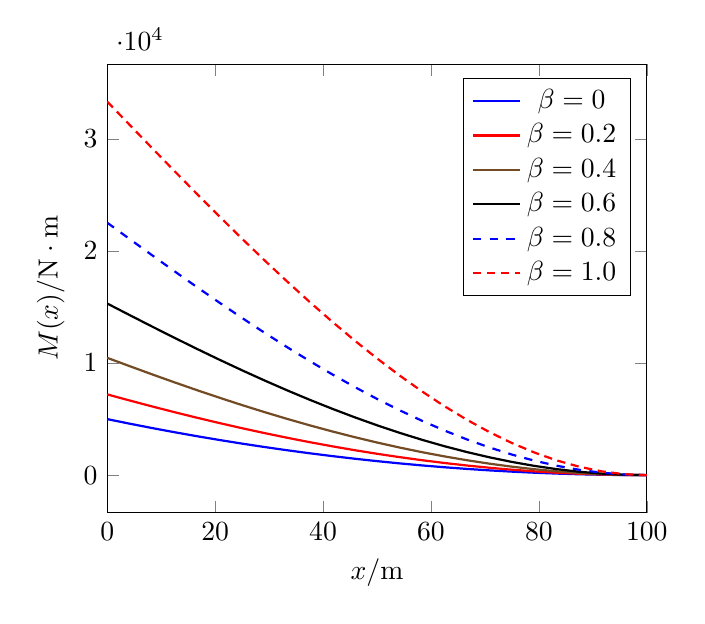
\begin{tikzpicture}
            \begin{axis}[
            xlabel={$x/\si{\m}$}, 
            ylabel={$M(x)/\si{N\cdot m}$}, 
            xmin=0,xmax=100,
            legend entries={$\beta=0$, $\beta=0.2$, $\beta=0.4$, $\beta=0.6$, $\beta=0.8$, $\beta=1.0$},%page255
            legend pos=north east,%page258
            ] 
            \addplot+[thick, no marks, domain=0:100] {1/2*x^2-100/1*x+(1 * 100^2)/2}; 
            \addplot+[thick, no marks, domain=0:100] {(10^(-0.2))/(1.2*2.2)*x^2.2-(10^(-0.2)*100^1.2)/1.2*x+(10^(-0.2) * 100^2.2)/2.2};
            \addplot+[thick, no marks, domain=0:100] {(10^(-0.4))/(1.4*2.4)*x^2.4-(10^(-0.4)*100^1.4)/1.4*x+(10^(-0.4) * 100^2.4)/2.4};
            \addplot+[thick, no marks, domain=0:100] {(10^(-0.6))/(1.6*2.6)*x^2.6-(10^(-0.6)*100^1.6)/1.6*x+(10^(-0.6) * 100^(2.6))/(2.6)};
            \addplot+[thick, no marks, domain=0:100, blue, dashed] {(10^(-0.8))/(1.8*2.8)*x^2.8-(10^(-0.8)*100^1.8)/1.8*x+(10^(-0.8) * 100^2.8)/2.8};
            \addplot+[thick, no marks, domain=0:100] {0.1/6*x^3-500*x+(1e5)/3};
            \end{axis}
        \end{tikzpicture}
        \stepcounter{pgfplots}\caption{\pgfcaption}
        \label{fig:pgfplots2}
    \end{figure}

    \begin{figure}[H]
        \centering
        \begin{tikzpicture}
        \begin{axis}[
        xlabel={$\beta$}, 
        ylabel={$H_{\max}/\si{\m}$}, 
        xmin=0,xmax=1,
        ] 
        \addplot+[thick, no marks] table {data/push.dat}; 
        \end{axis}
        \end{tikzpicture}
        \stepcounter{pgfplots}\caption{\pgfcaption}    
        \label{fig:pgfplots3}
    \end{figure}

    \begin{figure}[H]
        \centering
        \begin{tikzpicture}
        \begin{axis} [
        x dir=reverse,%page327
        xlabel={$F_2/\si{\N}$},
        ylabel={$\theta/\si{degree}$},
        zlabel={截面最大拉应力 $\sigma_m/\si{Pa}$},
        ytick={1.00000000e-05, 3.92709082e-01, 7.85408163e-01, 1.17810725e+00,
            1.57080633e+00, 1.96350541e+00,2.356194490192344837e+00},%page332
        yticklabels={ ,$22.5$,$45$,$67.5$,$90$,$112.5$,$135$},%page338
        minor ytick={1.57},%page335
        grid=minor,
        extra z ticks={149e6},%page336
        extra z tick style={grid=major},
        extra z tick labels={$\sigma_b$}
        %colormap/viridis,
        %colorbar,
        %view/h=40,
        ]
        \addplot3 [ 
        surf, 
        ] table {data/3dmap.dat}; 
        \end{axis}
        \end{tikzpicture}
        \stepcounter{pgfplots}\caption{\pgfcaption}
        \label{fig:pgfplot4}
    \end{figure}

    \begin{figure}[H]
        \centering
        \begin{tikzpicture}
        \begin{axis} [
        view={0}{90},%page308
        %x dir=reverse,
        ytick={1.00000000e-05, 3.92709082e-01, 7.85408163e-01, 1.17810725e+00,
            1.57080633e+00, 1.96350541e+00,2.356194490192344837e+00},
        yticklabels={ ,$22.5$,$45$,$67.5$,$90$,$112.5$,$135$},
        xlabel={$F_2/\si{\N}$},
        ylabel={$\theta/\si{degree}$},
        zlabel={截面最大拉应力},
        minor ytick={1.57},%page335
        grid=minor,
        %colormap/viridis,
        colorbar,%page280
        %view/h=40,
        ]
        \addplot3 [ 
        surf,%page136
        shader=interp,%page138
        ] table {data/3dmap.dat}; 
        
        \end{axis} 
        \end{tikzpicture}
        \stepcounter{pgfplots}\caption{\pgfcaption}
        \label{fig:pgfplots5}
    \end{figure}

    \begin{figure}[H]
        \centering
        \begin{tikzpicture}% file
        \begin{axis}[
        xlabel=n,
        ylabel=Orbits $/\si{AU}$,
        legend pos=north west,
        xmin=0, xmax=10,
        ymin=0, ymax=35, 
        ]
        \addplot+[smooth,thick,mark size=1.2pt] table {data/9.txt};
        \addplot+[thick,mark size=2pt, domain=0.9:9.1, no marks,samples=500] {-0.3304+0.2392*1.716^x}
        node [pos=0.3, pin=120:{$y=-0.3304+0.2392\times1.716^x$}] {};
        \addlegendentry{Data Measured}
        \addlegendentry{Fitted curve}
        \end{axis}
        \end{tikzpicture}
        \stepcounter{pgfplots}\caption{\pgfcaption\ (Fitted curve with $R^2=0.9957$)}
        \label{fig:pgfplots7}
    \end{figure}

    \begin{figure}[H]
        \centering
        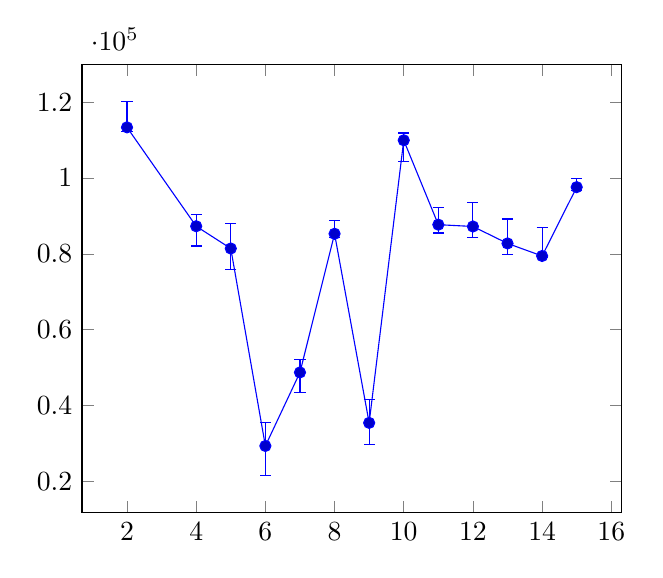
\begin{tikzpicture}
        \begin{axis}
        \addplot+[
        mark size=2pt,
        error bars/.cd, %page314
        y dir=both, y explicit, 
        ] table [
        y error plus=ey+,
        y error minus=ey-,
        ] {
            x y ey- ey+
            2 113341.2813019057 1100.611156427621609 6800.2713230942609
            4 87272.97693111458 5200.46801444790617 3190.1334855520836
            5 81404.46225000001 5500.19754166666826 6690.1267500000104
            6 29349.665352065687 7700.83223126764278 6210.0162312676475
            7 48737.92350537173 5300.63117203840375 3300.79170296161465
            8 85289.40943116492 1100.805764498276403 3560.7786105017585
            9 35436.53862314356 5600.200831476890016 6270.5355435231031
            10 109935.0145416667 5500.05712500003574 1930.70562499997322
            11 87686.45068919969 2200.665772533015115 4500.2008524670091
            12 87210.13071517028 2800.177215170275304 6230.1177431630786
            13 82739.89686456807 3000.464072901391773 6450.6765520985937
            14 79433.15006215085 300.9175204841740197 7610.7511045158171
            15 97579.32356719024 1000.348067190250731 2280.52818280975043
        }; 
        \end{axis} 
        \end{tikzpicture}
        \stepcounter{pgfplots}\caption{\pgfcaption}
        \label{fig:pgfplots8}
    \end{figure}

    \begin{figure}[H]
        \centering
        \begin{tikzpicture}
        \begin{axis}[variable=x, xlabel=波长$\si{/\nm}$, ylabel=折射率, legend pos=north east]
        \addplot[domain=420:750,blue,thick,samples=400]
        {sqrt(4.1366-1.0528e-6*x^2-7.9514e5*x^(-2)+2.1511e11*x^(-4)-2.6573e16*x^(-6)+1.2545e21*x^(-8))};
        \addplot+[only marks,thick]
        coordinates
        {
            (447.1,1.6705) (471.3,1.6654) (492.2,1.6612) (501.6,1.6596) 
            (587.6,1.6484) (667.8,1.6425) (706.6,1.6395)
        };
        \addlegendentry{回归曲线}
        \addlegendentry{原始数据}
        \end{axis}
        \end{tikzpicture}
        \stepcounter{pgfplots}\caption{\pgfcaption}
        \label{fig:pgfplots9}
    \end{figure}

    \begin{figure}[H]
        \centering
        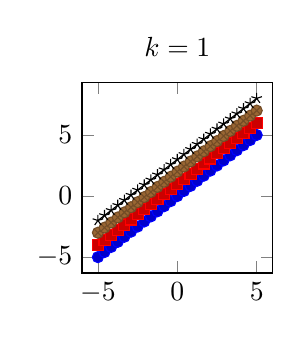
\begin{tikzpicture}
        \begin{axis}[
        legend columns=-1,
        legend entries={$(x+0)^k$;,$(x+1)^k$;,$(x+2)^k$;,$(x+3)^k$},
        legend to name=named,
        title={$k=1$},
        width=0.33\linewidth,
        height=0.33\linewidth,
        ]
        \addplot {x};
        \addplot {x+1};
        \addplot {x+2};
        \addplot {x+3};
        \end{axis}
        \end{tikzpicture}
        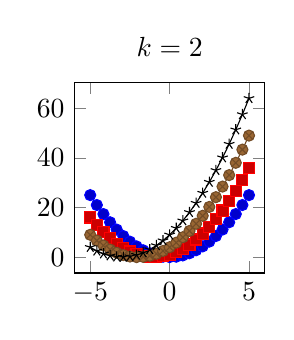
\begin{tikzpicture}
        \begin{axis}[title={$k=2$},
        width=0.33\linewidth,
        height=0.33\linewidth,]
        \addplot {x^2};
        \addplot {(x+1)^2};
        \addplot {(x+2)^2};
        \addplot {(x+3)^2};
        \end{axis}
        \end{tikzpicture}
        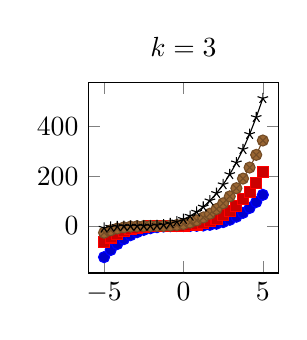
\begin{tikzpicture}
        \begin{axis}[title={$k=3$},
        width=0.33\linewidth,
        height=0.33\linewidth,]
        \addplot {x^3};
        \addplot {(x+1)^3};
        \addplot {(x+2)^3};
        \addplot {(x+3)^3};
        \end{axis}
        \end{tikzpicture}
        \\
        \ref{named}
        \stepcounter{pgfplots}\caption{\pgfcaption}
        \label{fig:pgfplots10}
    \end{figure}

    \begin{figure}[H]
        \centering
        \begin{tikzpicture}% file
        \begin{axis}[
        xlabel=环己烷\si{/\percent},
        ylabel=温度\si{/\celsius},
        xmin=-3, xmax=101, 
        ymin=60, ymax=85,
        minor xtick={0,100},%page335
        grid=minor,
        ]
        \addplot+[thick,no marks, red] table {data/gas_pretty.txt};
        \addplot+[only marks, mark=square*, red] table {data/gas.txt};
        \addplot+[smooth, thick, no marks,blue] table {data/liquid_pretty.txt};
        \addplot+[only marks, mark=*, blue] table {data/liquid.txt};
        \end{axis}
        \end{tikzpicture}
        \stepcounter{pgfplots}\caption{\pgfcaption}
        \label{fig:pgfplots11}
    \end{figure}

    \begin{figure}[H]
        \centering
        \begin{tikzpicture}% file
        \begin{axis}[
        xlabel=pH,
        ylabel=$\varepsilon \si{/\V}$,
        legend pos=south west,
        extra x ticks={6.5,8},
        extra tick style={grid=major},
        %xmin=1100, xmax=8400,
        %ymin=-4, ymax=5, 
        ]
        \addplot+[smooth,thick,mark size=1.2pt] table {data/1.txt};
        \addplot+[thick,mark size=1.5pt, domain=2.5:8, no marks] {-0.072+0.0296*5.00770-0.0591*x};
        \node [pin=above:{$(3.88,-0.1105)$}] at (3.88,-0.1105) {};
        \node [pin=above:{$(5.61,-0.1140)$}] at (5.61,-0.1140) {};
        \addlegendentry{$\ce{Fe^3+}/\ce{Fe^2+}$-$\mathrm{EDTA}$ 体系}
        \addlegendentry{$\ce{S}/\ce{H2S}$ 体系}
        \end{axis}
        \end{tikzpicture}
        \stepcounter{pgfplots}\caption{\pgfcaption}
        \label{fig:pgfplots12}
    \end{figure}

\end{document}